\documentclass[dvisvgm,border=2pt]{standalone}
% Shared by every figure. Two colours only: black becomes the text colour of
% whatever theme the app is in, and `accent` becomes the brand — see
% scripts/build-figures.mjs. Everything else is done with opacity.
\usepackage{amsmath}
\usepackage{amssymb}
\usepackage{tikz}
\usepackage{pgfplots}
\pgfplotsset{compat=1.18}
\usetikzlibrary{arrows.meta,positioning,calc,backgrounds,fit,patterns.meta}
\definecolor{accent}{RGB}{255,0,255}
\pgfplotsset{
  every axis/.append style={
    axis lines=left,
    axis line style={draw opacity=0.35},
    tick style={draw opacity=0.35},
    tick label style={font=\scriptsize,opacity=0.7},
    label style={font=\scriptsize,opacity=0.7},
    legend style={draw=none,fill=none,font=\scriptsize},
    every axis plot/.append style={line width=0.7pt},
  },
}
\tikzset{
  every picture/.style={font=\scriptsize},
  faint/.style={opacity=0.3},
  quiet/.style={opacity=0.55},
  box/.style={draw,opacity=0.35,rounded corners=2pt,inner sep=4pt},
  hot/.style={accent},
}

\begin{document}
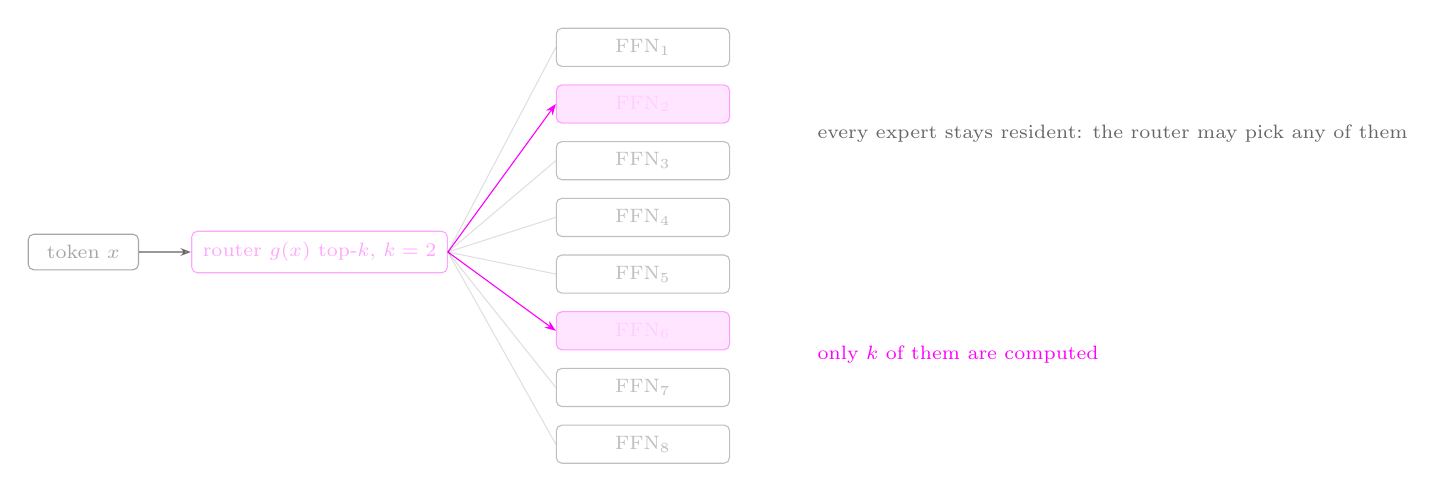
\begin{tikzpicture}[every node/.style={font=\scriptsize}]
  \node[box,minimum width=14mm] (tok) at (0,0) {token $x$};
  \node[box,draw=accent,text=accent,minimum width=20mm,align=center] (r) at (3,0)
    {router $g(x)$\ top-$k$, $k=2$};
  \draw[opacity=0.4,-{Stealth[length=4pt]}] (tok) -- (r);
  \foreach \i [count=\n from 0] in {1,...,8}{
    \pgfmathsetmacro{\y}{2.6-\n*0.72}
    \ifnum\i=2
      \node[box,draw=accent,text=accent,fill=accent,fill opacity=0.1,minimum width=22mm,anchor=west] (e\i) at (6,\y) {$\mathrm{FFN}_\i$};
      \draw[accent,-{Stealth[length=4pt]}] (r.east) -- (e\i.west);
    \else
      \ifnum\i=6
        \node[box,draw=accent,text=accent,fill=accent,fill opacity=0.1,minimum width=22mm,anchor=west] (e\i) at (6,\y) {$\mathrm{FFN}_\i$};
        \draw[accent,-{Stealth[length=4pt]}] (r.east) -- (e\i.west);
      \else
        \node[box,opacity=0.25,minimum width=22mm,anchor=west] (e\i) at (6,\y) {$\mathrm{FFN}_\i$};
        \draw[opacity=0.12] (r.east) -- (e\i.west);
      \fi
    \fi
  }
  \node[opacity=0.6,align=left,anchor=west] at (9.2,1.5) {every expert stays\ resident: the router\ may pick any of them};
  \node[accent,align=left,anchor=west] at (9.2,-1.3) {only $k$ of them\ are computed};
\end{tikzpicture}
\end{document}
